\section{Pilot Application}

In this network environment, we focus on consumer-facing applications, as shown in Figure~\ref{fig:continuum}. 
Mobile physical activity monitoring applications
(fitness tracker) with location-based content push.

For our use case, focus on a \textbf{simple ecosystem of composable services rather than a single siloed application.}

Our pilot application:  \textbf{NDNEx} (NDN-Exercise) and a user-facing \textbf{Identity Manager}.  Supporting physical activity is both a critical part of building healthy communities and a key retail market. 

Our objective is not only an application.

It is to act as an example of interoperating components of an Open mHealth ecosystem.

This places additional requirements on the design.

See Deborah's TEDMED talk: 
\url{https://www.youtube.com/watch?feature=player_embedded&v=lAEhSGYEHWU}


\begin{figure*}
\begin{center}
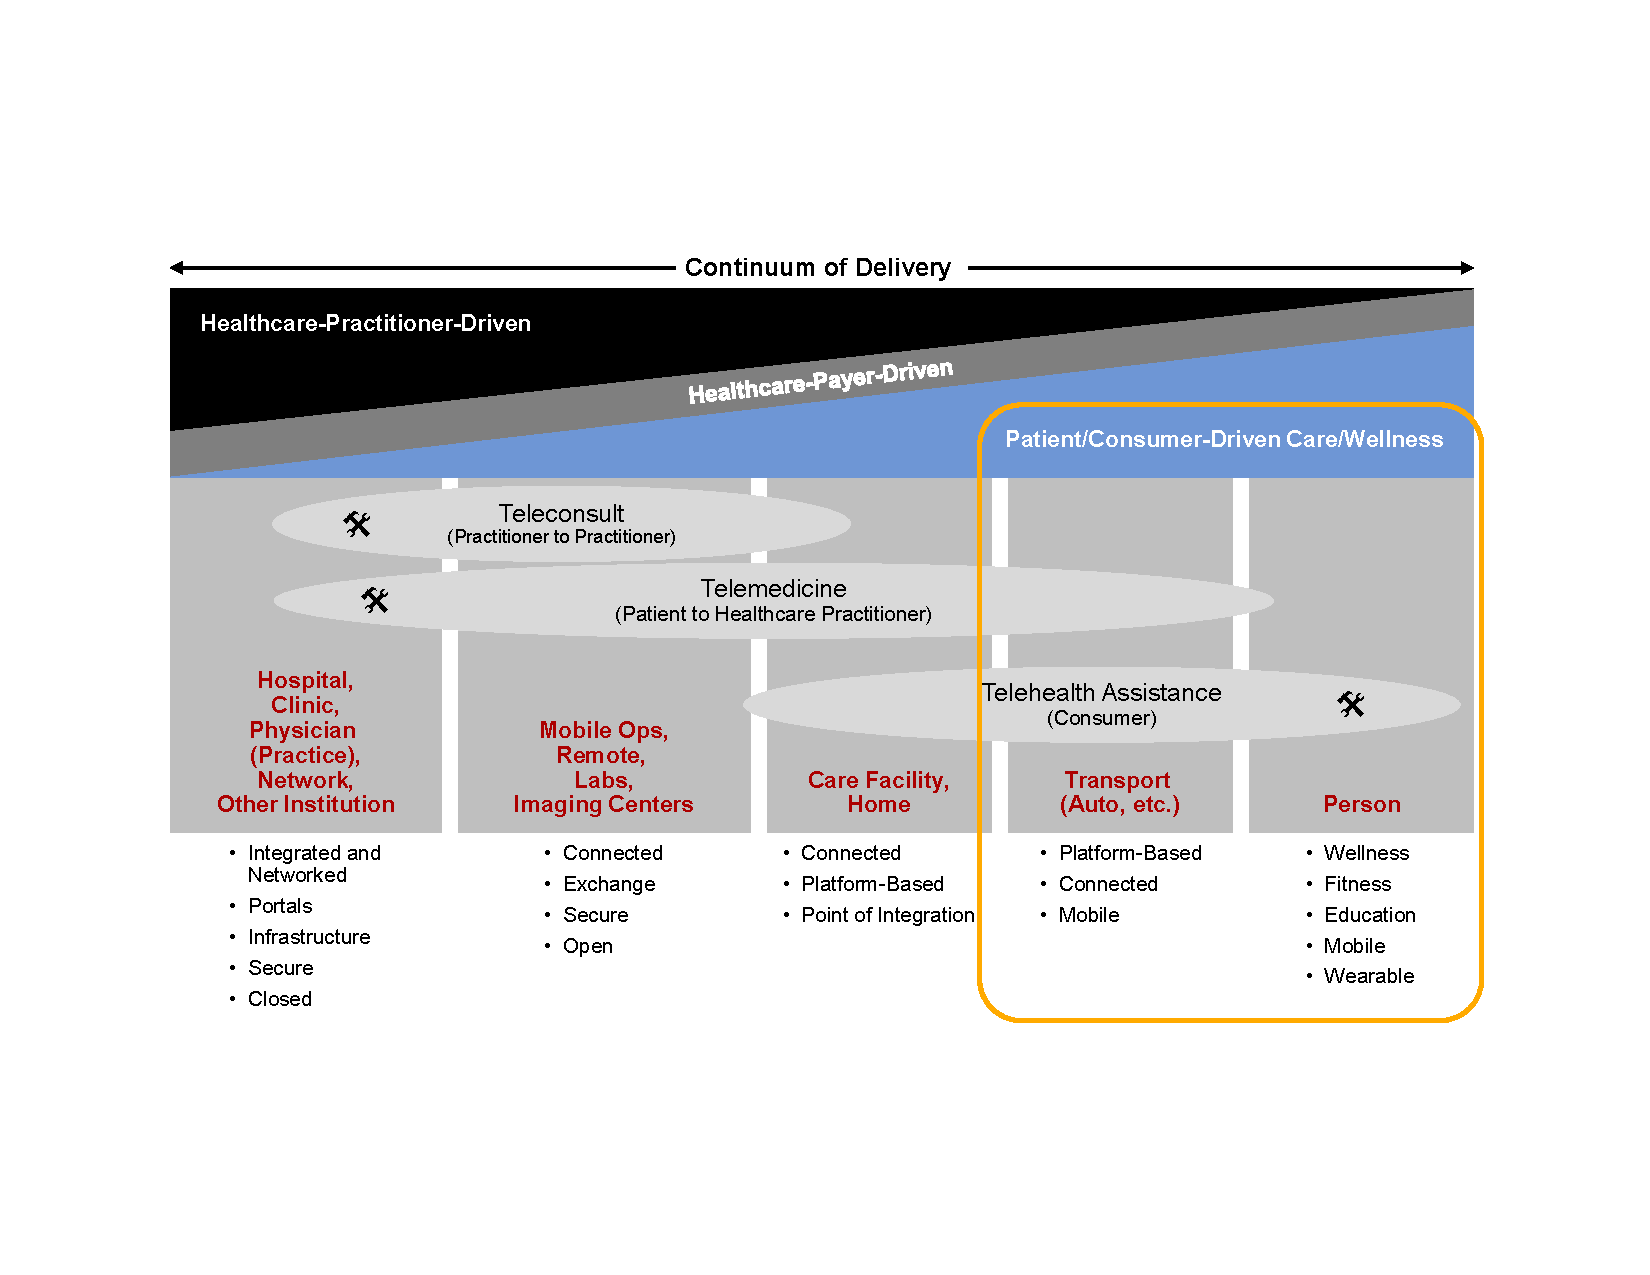
\includegraphics[width=.8\textwidth]{figures/continuum}
\caption{{Focus of Open mHealth network environment shown in yellow box. Figure from Gartner, 2013.  }}
% A Framework for Understanding Telehealth, Telemedicine and Other Remote Healthcare Delivery Solutions
% need to redraw before release
\label{fig:continuum}
\end{center}
\end{figure*}


NDNEx is a non-proprietary ecosystem for consumer physical activity data. 

Start with end-user mobile+web application that captures and reports walking, jogging, and running activity.

Calculate and report activity metrics based on GPS and accelerometer data  both automatically and self-identified rounds of exercise.  

Ad-hoc and formal groups or teams. 

Capable of location-based content push during the exercise, which can be used for health, entertainment, local, and team-related content. 

Commercial parallels:  Nike+, Fitbit, Endomondo (see Figure~\ref{fig:endomondo}), etc. 

\begin{figure}
\begin{center}
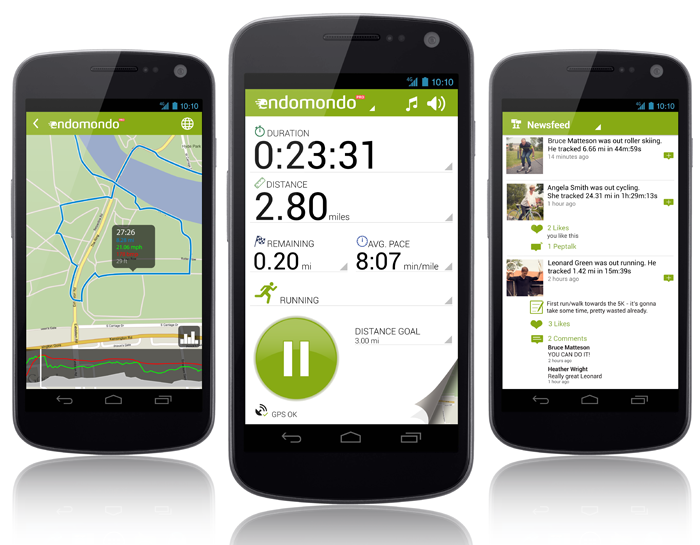
\includegraphics[width=.6\textwidth]{figures/endomondo}
\caption{Endomondo commercial fitness tracker. \protect\url{https://www.endomondo.com/}}
\label{fig:endomondo}
\end{center}
\end{figure}


Envisioned as an open-data ecosystem, with different service providers at different stages in the processing chain, rather than a siloed application.

Work that we can leverage (see related work above): 

Open mHealth Toolset  including Ohmage reference platform and the Lifestreams concept. 

Past CENS/UCLA participatory sensing research in activity classification,self-surveillance privacy, mobile phone based data collection.

REMAPs funded collaborations on Urban Trails and technology for Parks with California State Parks, the Western National Parks Association, National Park Service, and the City of Los Angeles. 

\begin{figure}
\begin{center}
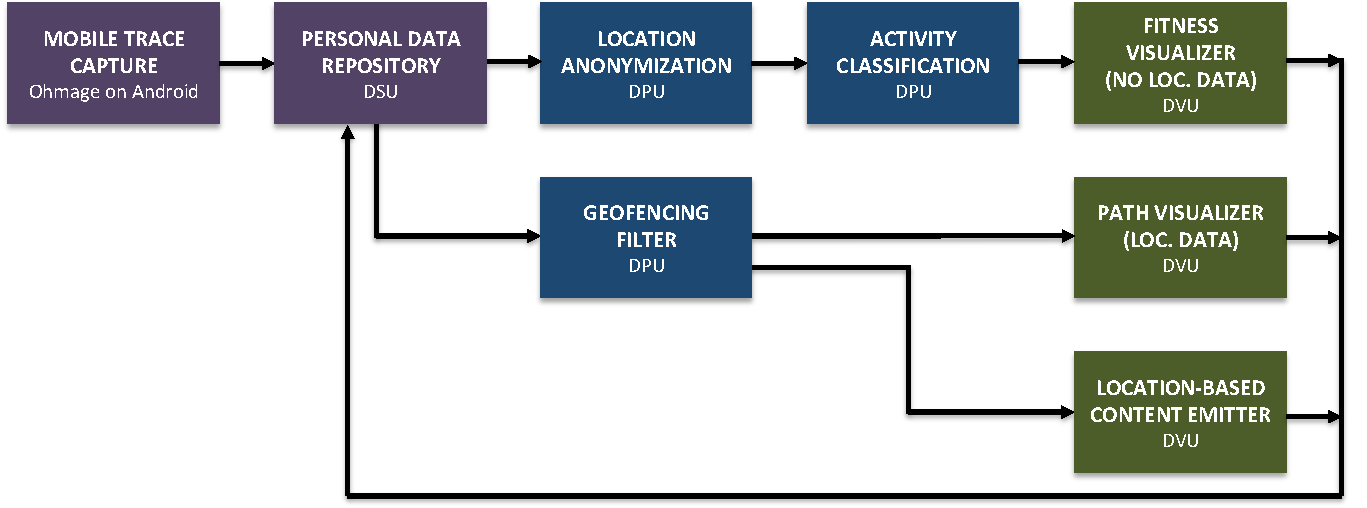
\includegraphics[width=1\textwidth]{figures/ConceptualBlock}
\caption{Conceptual block diagram showing data flow.}
\label{fig:ConceptualBlock}
\end{center}
\end{figure}


\subsection{Research Objectives} 

{\bf Naming and application design.} The Open mHealth architecture focuses on data exchange rather than system interoperability, which is well-suited for NDN. Using NDN rather than IP enables Open mHealth applications to be coded using data naming directly rather than having to create abstractions to translate data names to IP-based hosts providing services. We will explore how application architecture can be simplified and map closely to network architecture. With its emerging synchronization primitives, NDN will also enhance network support for synchronizing data across multiple devices. 

{\bf Trust and security.} Because NDN does not rely on perimeter- or channel-based security, it will promote global health data ecosystems rather than previous walled garden approaches.   This shift has direct relevance for public health, by enabling research to draw from large populations. 

{\bf Storage in the network.} NDN naturally supports distributed storage, which can ease the burden of fault-tolerance and load-balancing in large networks, reducing cost-of-entry and fostering innovation. 


\subsection{Existing Building Blocks} 

What we will leverage to build this application.

\paragraph{What to keep from current Open mHealth design.}
\begin{itemize}
\item Data-centric rather than service-centric interoperability. $\Rightarrow$ \emph{Focus on data namespace design.}
\item Distributed architecture of Capture, DSU, DPU, DVU. $\Rightarrow$ \emph{Implement data flow approach in NDN.}
\item End user focus (not hospitals, doctors, etc.) $\Rightarrow$ \emph{Consumer app deployment scenario.}
\item User-centric privacy approach. $\Rightarrow$ \emph{Need to inform user of choices, data flow.}
\item Encrypted communications. $\Rightarrow$ \emph{Encryption-based access control, name encryption.}
\item Mobile publishing. $\Rightarrow$ \emph{Use as our driver to solve this oft-cited challenge.}
\end{itemize}

\paragraph{What to discard from current Open mHealth design.}
\begin{itemize}
\item REST/HTTP: Move away from RPC call model and carrying state in Interests.
\item Host-based endpoints for services:  focus on data dissemination model and NFN style processing. 
\item OAuth: need new identity / authentication support. 
\item Single storage ``location''. 
\end{itemize}


\subsubsection{Capture: Ohmage \& Mobility}

\url{http://ohmage.org/}

ohmage is an open-source participatory sensing technology platform. It supports: 1) expressive project authoring; 2) mobile phone-based data capture through both inquiry-based surveys and automated data capture as well as temporally and/or spatially triggered reminders, 3) data visualization and real-time feedback; privacy respecting data management; and 4) extensible data exploration. 

Tangmunarunkit, H., et al. "Ohmage: A General and Extensible End-to-End Participatory Sensing Platform,” ACM Trans. on Intelligent Systems and Technology (in submission), UCLA CS Technical Report 140015. (Used in 20 projects.)  \url{http://web.ohmage.org/~hongsudt/pub/ohmage_ucla_140015.pdf}



\subsubsection{Storage: Open mHealth Data Storage Unit (DSU) Design}

\url{https://github.com/openmhealth/developer/wiki/DSU-Overview}

The Open mHealth DSU (Data Storage Unit) API Specification is an open specification for unified information sharing across disparate data streams. The idea is simple: create an easy-to-understand set of APIs that allow siloed data stores to share information. Third-party applications that understand this API specification can then create a single set of tools to access data across any of the servers.


\subsubsection{Storage: Personal Data Vault} 

Reference Derek's work here? 

Mun, Min, et al. "Personal data vaults: a locus of control for personal data streams." Proceedings of the 6th International Conference. ACM, 2010.http://remap.ucla.edu/jburke/publications/Mun-et-al-2010-Personal-Data-Vaults.pdf

Kang, J., Shilton, K., Estrin, D., Burke, J. "Self-surveillance privacy." Iowa L. Rev. 97 (2011): 809.http://escholarship.org/uc/item/1jk8b2q1.pdf

\subsubsection{Processing: Open mHealth Data Processing Unit (DPU) Design}

\url{https://github.com/openmhealth/developer/wiki/Open-mHealth-and-Data-Processing}

DPUs are stateless modules that input and output data. They are designed to be embedded in other software or called remotely. They do not produce anything directly visible, but are the brains and muscles of an application. The concept of a DPU is inspired by the Unix Philosophy of creating small functional tools that can be chained and reused, rather than a single large application.

\subsubsection{Processing: Named Function Networking Concept}

\url{http://www.named-function.net/}

Names serve to access and invoke functions, which incidentally can produce passive content once it is needed. New questions arise from this point of view, namely how the network organizes the flow of functions, which brings us squarely into active networking turf. 

Initially, focusing on location-based triggers (geofencing) - to trigger location-based content.

\subsubsection{Analytics / Presentation: Ohmage Front-end for Mobilize}

\url{https://wiki.mobilizingcs.org/app/web}

The web frontend (powered by the ohmage project) is used to provide students secure access to their data. It supports secure login, campaign management, data management and basic campaign monitoring and visualization. The students can review and share their data to the growing data set collected by their class. The web frontend can also be used to discover the answers to basic statistical inferences in real-time as data is being collected. When data collection is complete, the web frontend allows for easy exporting of the data to a more thorough statistical analysis tool. 

\subsubsection{Analytics / Presentation: Lifestreams Dashboard}

\cite{hsieh2013acm}

\subsubsection{Content push: Trails Database}

\url{http://archinect.com/news/article/111897927/tour-los-angeles-history-with-ucla-s-new-interactive-urban-trail-app}

The LASHP Trails Mobile Website gives residents and visitors to Northeast Downtown Los Angeles site-specific access to a dynamic combination of historic information and health-related activities along urban trails starting and ending at the Los Angeles State Historic Park. 

\subsection{Application Requirements}

Summarize. 

The Open mHealth team envisions that the Internet will interconnect 1)
data capture, 2) secure storage, 3) modeling and analytics, and 4) user
interface components to create a modular, layered sense-making framework.  
%% Repeated from above.

Adaptation of Open mHealth REST-based communication model to a data dissemination approach inspired by NDN.

\subsubsection{Naming} 
\begin{itemize}
\item \textbf{Data format namespace design} comes directly from Open mHealth developer documentation. 
\item \textbf{Application architecture} consistent with the pieces above and from previous participatory sensing projects. (e.g., Mun et al, 2009)
\item What schema? Initially, try direct mapping of Open mHealth schema
\item Borrow ideas from Named Function Networking concept for distributed processing
\item Translate existing REST-based approach or do pure NDN? 
\item Represent raw time-location data (GPS, accelerometer) from mobiles. 
\item Support successive rounds of processing that, for example:  
    \begin{itemize}
    \item Generate classified activity data that follows the Physical Activity JSON schema and perhaps other related schemas.  (This happens at client-side in Ohmage Mobility but could happen at a DPU.)	
    \item Identify / segment ``bouts”''of physical activity or exercise. 
    \item Add features to a bout from DPUs to the existing store. 
    \end{itemize}
\item Consumers should be able to access raw and processed data for a certain time period.
\item Consumers should be able to efficiently read data sequentially. 
\end{itemize}

\subsubsection{Trust and security}

Fit NDN architectural mechanisms into security requirements
\begin{itemize}
\item \textbf{Identity and trust management} scenario comes from our proposed application use case.  (Recall:  Not just an app, an example of interoperating components in an ecosystem.)
\item Provide granular access control over various components of the data namespace – in particular, raw location data. 
\item Replacing Oauth2 for distributed processing is critical
\item Data encryption requirements
\item Name privacy issues
\item Follow passive key publication approach (rather than active) if possible. 
\end{itemize}
Can / should we support different identities relative each part of the system: collection, processing, and visualization?
Collection: User may publish data to serve multiple applications, but doesn’t want them to be able to conspire / correlate that they are the same user.
Processing:  Design should provide the minimum possible information to the processing components about user identity. 
Visualization: Visible face of “the app” to the user. 

\subsubsection{Storage in the network}
\begin{itemize}
\item Interaction of personal and shared stores
\item Data filtering at the repo?
\item New legal / economic relationship between the players
\end{itemize}
